%% main_rtai_artigo.tex, based on abtex2-modelo-Artigo.tex, v-1.9.6 laurocesar 
%% Adaptado por Prof. Dr. Renato Kazuo Miyamoto 
%% Departamento de Elétrica e Automação
%% Centro Universitário UNISENAI Londrina

%% Copyright 2012-2016 by abnTeX2 group at http://www.abntex.net.br/ 

% ------------------------------------------------------------------------
% ------------------------------------------------------------------------
% abnTeX2: Modelo de Artigo Acadêmico em conformidade com
% ABNT NBR 6022:2003: Informação e documentação - Artigo em publicação 

% ------------------------------------------------------------------------
% ------------------------------------------------------------------------

\documentclass[
% -- opções da classe memoir --
article,			% indica que é um artigo acadêmico
11pt,				% tamanho da fonte
twoside,			% para impressão apenas no recto. Oposto a twoside
a4paper,			% tamanho do papel
% -- opções da classe abntex2 --
%chapter=TITLE,		% títulos de capítulos convertidos em letras maiúsculas
section=TITLE,		% títulos de seções convertidos em letras maiúsculas
%subsection=TITLE,	% títulos de subseções convertidos em letras maiúsculas
%subsubsection=TITLE % títulos de subsubseções convertidos em letras maiúsculas
% -- opções do pacote babel --
onecolumn,          % texto em duas colunas
english,			% idioma adicional para hifenização
brazil,				% o último idioma é o principal do documento
sumario=tradicional
]{abntex2}

\usepackage{sty/packs}

% ----
% Se necessário, inclua outros pacotes aqui
\usepackage[utf8]{inputenc}
\usepackage{hyperref}
\usepackage{graphicx}
\usepackage[alf]{abntex2cite}	% Citações padrão ABNT
\usepackage{footmisc} % para melhorar formatação das notas de rodapé
% ---
\begin{document} 
% ---
% Informações de dados para CAPA e FOLHA DE ROSTO
% ---
% Título
\begin{center}
   
    {\bfseries TÍTULO: subtítulo em língua vernácula} \\
   
    \vspace{0.5cm}

\end{center}



% Autores alinhados à direita
\begin{flushright}
    \fontsize{7}{9}\selectfont
    Angelo Aparecido Salvador Avelino\footnotemark[1] \quad   \\
    Gabriel Gonçalves Costa\footnotemark[2] \quad \\
    Huan Radov Luchetti\footnotemark[3] \quad  \\
    Lucas Vinicius de Bortoli Santos\footnotemark[4] \quad  \\
    Pedro Antônio Frasson\footnotemark[5] \quad  \\
    Vinicius de Morais Boim dos Santos\footnotemark[6] \quad  \\
    Cinthya Oestreich Silva (Orientador)\footnotemark[7] \\
\end{flushright}

\vspace{1cm}

% Definindo as notas de rodapé para cada autor
\footnotetext[1]{UniSENAI PR, angeloavelino33211781@gmail.com}
\footnotetext[2]{UniSENAI PR, gab.gabriel.1003@outlook.com)}
\footnotetext[3]{UniSENAI PR, pafrasson@gmail.com)}
\footnotetext[4]{UniSENAI PR, lucasbortolisantos@gmail.com)}
\footnotetext[5]{UniSENAI PR, huan.luchetti@gmail.com)}
\footnotetext[6]{UniSENAI PR, vinicius.santos00857469@sesisenaipr.org.br)}
\footnotetext[7]{UniSENAI PR, cinthya.silva@docente.senai.br)}

\vspace{1cm}

%\local{Brasil}
%\data{ Departamento de Engenharia Elétrica e Automação Industrial \\ Centro Universitário UniSenai PR \\ Londrina/PR - Brasil - Janeiro 2025, v-1.0}
% ---

% ----
% Início do documento
% ----

    
% Seleciona o idioma do documento (conforme pacotes do babel)
%\selectlanguage{english}
\selectlanguage{brazil}

% Retira espaço extra obsoleto entre as frases.
\frenchspacing 

% ----------------------------------------------------------
% ELEMENTOS PRÉ-TEXTUAIS
% ----------------------------------------------------------

%\twocolumn[    		% INICIO DE ARTIGO EM DUAS COLUNAS
% página de titulo
% \maketitle
% resumo em português
\begin{resumo}
    A Internet das Coisas (IoT) tem revolucionado a forma como dispositivos e sistemas são conectados, permitindo a criação de ambientes inteligentes e integrados, como as Cidades Inteligentes. Essas cidades dependem da comunicação eficiente entre dispositivos distribuídos para otimizar recursos, melhorar a segurança e facilitar o controle remoto de infraestrutura crítica. No entanto, a conectividade remota de dispositivos físicos ainda enfrenta desafios significativos em regiões com infraestrutura de rede limitada, onde custos elevados e baixa acessibilidade dificultam a implementação de soluções eficientes. Tecnologias como LoRa, que oferecem comunicação de longo alcance com baixo consumo energético, surgem como alternativas viáveis para superar essas barreiras. Este trabalho apresenta uma solução baseada em LoRa e MQTT para o controle remoto de cancelas de estacionamento, utilizando módulos ESP32 com comunicação LoRa e um gateway que integra a rede local a um servidor MQTT. A arquitetura proposta permite que comandos sejam enviados e executados de qualquer lugar com acesso à internet, garantindo baixo custo, segurança e escalabilidade.

    \noindent
    \textbf{Palavras-chave}: IoT. LoRa. Computação de Ponta. Cidades Inteligentes.
\end{resumo}
    
% resumo em inglês
\renewcommand{\resumoname}{Abstract}
\begin{resumo}
    \begin{otherlanguage*}{english}
        The Internet of Things (IoT) has revolutionized the way devices and systems are connected, enabling the creation of intelligent and integrated environments such as Smart Cities. These cities rely on efficient communication between distributed devices to optimize resources, enhance security, and facilitate remote control of critical infrastructure. However, remote connectivity of physical devices still faces significant challenges in regions with limited network infrastructure, where high costs and low accessibility hinder the implementation of effective solutions. Technologies like LoRa, which offer long-range communication with low power consumption, emerge as viable alternatives to overcome these barriers. This work presents a solution based on LoRa and MQTT for remote control of parking lot gates, using ESP32 modules with LoRa communication and a gateway that connects the local network to an MQTT server. The proposed architecture enables commands to be sent and executed from anywhere with internet access, ensuring low cost, security, and scalability.
        
        \noindent
        \textbf{Keywords}: IoT. LoRa. Edge Computing. Smart Cities.
    \end{otherlanguage*}  
\end{resumo}


\vspace{\onelineskip}%

% ----------------------------------------------------------
% ELEMENTOS TEXTUAIS
% ----------------------------------------------------------
\textual

% ----------------------------------------------------------
% Introdução
% ----------------------------------------------------------
\section{Introdução}
\addcontentsline{toc}{section}{Introdução}

    No contexto das Smart Cities, a Internet das Coisas (IoT) tem se destacado como uma tecnologia transformadora, permitindo a interconexão de dispositivos e sistemas para otimizar processos e melhorar a eficiência. A adoção de protocolos de comunicação eficientes é crucial para o sucesso dessas aplicações, especialmente em ambientes com conectividade limitada. Nesse cenário, o protocolo LoRa (Long Range) tem emergido como uma solução promissora devido à sua capacidade de comunicação de longo alcance com baixo consumo de energia \cite{Yoon2020}.

    Para maior versatilidade na transmissão de dados, a adoção de um gateway LoRa-MQTT (Message Queuing Telemetry Transport) tem se mostrado eficaz. O gateway atua como intermediário entre os dispositivos LoRa e a nuvem, facilitando a transmissão de dados de sensores e atuadores para plataformas de análise e monitoramento em tempo real \cite{Bhawiyuga2019}.

    A existência de edifícios pode interferir na comunicação LoRa, como ressalta \cite{lima2023}. Contudo, esse efeito pode ser minimizado com o uso de antenas de maior ganho e com o posicionamento estratégico dos dispositivos.

    Diante desse contexto, este artigo propõe o desenvolvimento de um sistema de controle remoto de cancelas de estacionamento utilizando a tecnologia LoRa e o protocolo MQTT. A solução visa permitir o gerenciamento eficiente e seguro das cancelas a partir de qualquer local com acesso à internet, oferecendo uma alternativa prática, de baixo custo e escalável para aplicações urbanas.

    Este trabalho busca atender a uma demanda apresentada pela empresa Estacenter, que busca uma solução de contingência para abertura de cancelas em estacionamentos inteligentes. O requisito consiste no desenvolvimento de um sistema modular e de baixo custo, capaz de operar mesmo em situações de falha de rede cabeada, utilizando conectividade via TCP/IP e LoRa.

    O artigo está organizado da seguinte forma: a Seção 2 descreve os fundamentos teóricos, a Seção 3 apresenta a arquitetura proposta, a Seção 4 discute os resultados e, por fim, a Seção 5 apresenta as conclusões.

% A introdução deve apresentar uma visão geral do artigo, delimitando o tema e o problema a ser abordado, bem como o (s) objetivo (s) e a justificativa. O intuito é chamar a atenção do leitor para o assunto que será apresentado no artigo, sem aprofundar conceitos ou antecipar resultados. 

% ----------------------------------------------------------
% Seção de explicações
% ----------------------------------------------------------
\section{Fundamentação Teórica}

    \subsection{Internet das Coisas (IoT)}
    A Internet das Coisas (IoT) consiste em um ecossistema de dispositivos interconectados capazes de coletar, processar e transmitir dados em tempo real, promovendo a integração entre o mundo físico e digital \cite{lima2023}. Esse paradigma é aplicado em diversos setores, como agricultura, cidades inteligentes e monitoramento ambiental. No entanto, ainda enfrenta desafios relacionados à escalabilidade, interoperabilidade entre dispositivos e limitações de consumo energético \cite{huh2019}. Nesse contexto, soluções de conectividade de baixo custo e baixo consumo surgem como alternativas promissoras para viabilizar a expansão da IoT.

    \subsection{LoRa}
    O protocolo LoRa (Long Range) é uma tecnologia de comunicação sem fio da categoria LPWAN (\textit{Low Power Wide Area Network}), que se destaca por oferecer grande alcance (até 15 km em áreas abertas) aliado ao baixo consumo de energia \cite{lima2023}. A modulação utilizada é baseada em espalhamento espectral por chirp (\textit{Chirp Spread Spectrum — CSS}), que garante maior robustez contra interferências. Já o protocolo LoRaWAN atua na camada de rede, fornecendo mecanismos de autenticação, criptografia e diferentes classes de dispositivos (A, B e C), possibilitando comunicação bidirecional e segura \cite{huh2019}. Apesar de suas vantagens, o LoRaWAN apresenta limitações, como a alta taxa de colisão de pacotes em cenários com muitos dispositivos transmitindo simultaneamente.

    \subsection{MQTT}
    O MQTT (Message Queuing Telemetry Transport) é um protocolo de comunicação leve, desenvolvido sobre TCP/IP, baseado no modelo \textit{publish-subscribe} \cite{Yoon2020}. Sua arquitetura envolve três elementos principais: \textit{publisher}, \textit{subscriber} e \textit{broker}. Esse protocolo se destaca por exigir baixa largura de banda, oferecer três níveis de Qualidade de Serviço (QoS) e garantir confiabilidade na entrega de mensagens em ambientes com restrições de energia e conectividade \cite{Bhawiyuga2019}. Devido a essas características, o MQTT é amplamente adotado em sistemas IoT que integram sensores, atuadores e plataformas em nuvem.

    \subsection{Aplicações Práticas}
    A combinação de LoRa e MQTT tem sido explorada em diferentes contextos práticos. Na aquicultura, Bhawiyuga et al. (2019) propuseram um sistema em que sensores de pH, oxigênio dissolvido e turbidez transmitem dados via LoRa para um gateway, que os encaminha para a nuvem através do MQTT \cite{Bhawiyuga2019}. Já no contexto agrícola, Yoon et al. (2020) desenvolveram a L\&M Farm, um sistema de irrigação inteligente que coleta dados de solo e clima, utilizando LoRa para comunicação entre sensores e atuadores, enquanto o MQTT garante a integração com aplicações web para tomada de decisão \cite{Yoon2020}. Esses estudos evidenciam o potencial da integração entre ambas as tecnologias para melhorar eficiência, reduzir custos e ampliar a automação em ambientes distribuídos.

    \subsection{ESP32}
    O microcontrolador ESP32 é amplamente utilizado em projetos IoT devido ao seu baixo custo, suporte a múltiplos protocolos de comunicação (Wi-Fi, Bluetooth e LoRa, em versões específicas), alta capacidade de processamento e baixo consumo energético \cite{lima2023}. A integração do ESP32 com módulos LoRa possibilita o desenvolvimento de protótipos de fácil implementação, capazes de transmitir dados em tempo real para plataformas de visualização e armazenamento. Testes práticos realizados por Lima (2023) demonstraram a capacidade de transmissão de dados em distâncias superiores a 10 km em ambientes abertos, ressaltando seu potencial para aplicações em áreas rurais e remotas.

    \subsection{Redes Mesh com LoRa}
    Embora o LoRaWAN tradicional adote uma topologia em estrela, pesquisas recentes indicam que sua aplicação em redes privadas pode enfrentar limitações de cobertura e confiabilidade. Nesse sentido, Huh e Kim (2019) propuseram uma versão modificada do protocolo, com suporte a redes \textit{mesh} e esquemas de múltiplo acesso para reduzir colisões de pacotes \cite{huh2019}. Em redes \textit{mesh}, cada nó pode atuar como roteador, aumentando a cobertura e permitindo rotas alternativas para transmissão de dados. Essa abordagem se mostrou eficaz em cenários como monitoramento ambiental em estaleiros e controle inteligente de iluminação pública, dispensando a necessidade de múltiplos gateways e reduzindo custos de infraestrutura.

\section{Metodologia}

    A metodologia aplicada neste trabalho compreende a modelagem da arquitetura, experimento para simular a implementação num cenário prático e por fim testes para avaliar o desempenho da solução.
    
    \subsection{Arquitetura Proposta}
    O sistema é composto por três cancelas experimentais, cada uma representada por um módulo ESP32 equipado com transceptor LoRa. Um dos dispositivos atua como \textit{gateway híbrido}, utilizando protocolo duplo, sendo TCP/IP para receber comandos do serviço web e LoRa para encaminhar a solicitação ao nó (cancela) correspondente. Os demais nós atuam como cancelas remotas, responsáveis por acionar fisicamente a saída digital que abre a cancela.

    \begin{figure}[htbp]
        \centering
        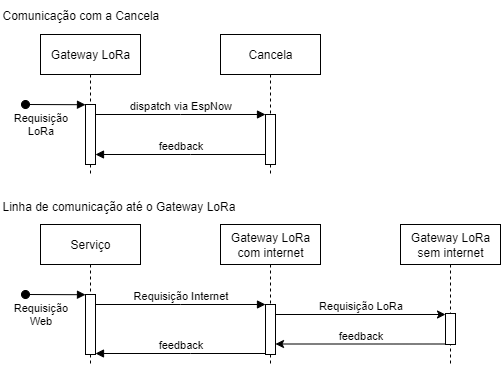
\includegraphics[width=0.9\linewidth]{Arquitetura.png}
        \caption{Fluxo de operação do sistema proposto para abertura de cancelas em estacionamentos.}
        \fonte{Elaborado pelos autores (2025).}
        \label{fig:fluxo_sistema}
    \end{figure}

    O processo de comunicação segue o fluxo:
    \begin{enumerate}
        \item O operador acessa um aplicativo móvel autenticado, seleciona a cancela desejada e envia o comando de abertura.
        \item O serviço web registra o log da operação em un banco de dados e envia a requisição ao gateway.
        \item O gateway recebe a mensagem via TCP/IP e a encaminha ao nó destino utilizando comunicação LoRa.
        \item O nó (cancela) aciona a saída digital e retorna um \textit{feedback} ao gateway, que repassa a confirmação ao sistema.
    \end{enumerate}
    
    \subsection{Dual-Protocol Networking}
    No sistema proposto, o gateway ESP32 foi configurado para operar como uma ponte entre dois protocolos distintos: TCP/IP e LoRa. 
    A comunicação entre o serviço web e o gateway ocorre via TCP/IP (utilizando Wi-Fi ou rede cabeada), garantindo integração com o aplicativo móvel e o banco de dados central. 
    Já a comunicação entre o gateway e os dispositivos que representam as cancelas é realizada por meio do protocolo LoRa, permitindo baixo consumo energético e maior alcance em cenários onde a infraestrutura de rede cabeada não está disponível.

    \subsection{Aplicativo Móvel}
    Foi desenvolvido um aplicativo móvel, no qual o usuário precisa realizar autenticação. Através desse aplicativo o usuário pode enviar comandos de abertura de cancela. Como o usuário está autenticado, o sistema tem controle de acesso e rastreabilidade, alinhando-se ao requisito da empresa de manter logs detalhados de operação.
    
    \subsection{Planejamento de Testes}
    Inspirando-se no trabalho recente \cite{rahmatullah2025}, previmos a necessidade dos seguintes testes para avaliar a solução:

    \begin{itemize}
        \item \textbf{Taxa de sucesso de entrega de pacotes}: análise da porcentagem de mensagens corretamente recebidas entre gateway e nós.
        \item \textbf{Atraso de transmissão (delay)}: tempo necessário entre o envio do comando pelo aplicativo e a execução na cancela.
        \item \textbf{Vazão (throughput)}: quantidade de dados transmitidos com sucesso em um intervalo de tempo.
        \item \textbf{Perda de pacotes (packet loss)}: proporção de pacotes perdidos em diferentes condições de distância e obstáculos.
        \item \textbf{Jitter}: variação do atraso de comunicação, que impacta a previsibilidade do sistema.
    \end{itemize}
    
    \subsection{Extensão com Comunicação Multinó}
    Queremos avaliar a possibilidade dos nós atuarem também como retransmissores, formando uma rede LoRa em topologia \textit{mesh} simplificada. Essa abordagem busca aumentar o alcance e a confiabilidade da comunicação em cenários onde o gateway não consegue contatar diretamente determinado nó. Contudo, conforme discutido em \cite{huh2019} \cite{rahmatullah2025}, essa configuração pode introduzir conflitos de recepção entre múltiplos nós e, portanto, serão necessários ajustes como escalonamento de tempo (\textit{time slots}) ou técnicas de mitigação de colisão.

% \section{Apresentação de discussão dos resultados}
%     Nessa seção devem constar os resultados encontrados na pesquisa, visando cumprir os objetivos propostos, através da metodologia especificada na seção anterior. É facultado ao autor dividir essa seção em subseções conforme ABNT NBR 6024 (2012). 
%     (Caso sua pesquisa seja uma Pesquisa Bibliográfica use como título desta seção apenas Discussão)



    % ---
    % Finaliza a parte no bookmark do PDF, para que se inicie o bookmark na raiz
    % ---
    \bookmarksetup{startatroot}% 
    % ---
    
    % ---
    % Conclusão
    % ---
    % \section{Considerações finais}
    % \addcontentsline{toc}{section}{Considerações finais}
    % Parte final do artigo, na qual o autor evidencia que os objetivos foram cumpridos, destaca os principais resultados obtidos e deixa sugestões para estudos futuros acerca do tema estudado.
    
    % Na conclusão não se utiliza citações, ilustrações e não se apresenta resultados ou conceitos novos (que não haviam sido apresentados anteriormente no texto).

    
        
    % ----------------------------------------------------------
    % ELEMENTOS PÓS-TEXTUAIS
    % ----------------------------------------------------------
    \postextual                 % Os elementos pós-textuais estão desabilitados nesse modelo
    
    % ----------------------------------------------------------
    % Referências bibliográficas
    % ----------------------------------------------------------
    \bibliography{rtai}
    
    % ----------------------------------------------------------
    % Glossário
    % ----------------------------------------------------------
    %\glossary
    
    % ----------------------------------------------------------
    % Apêndices
    % ----------------------------------------------------------
    % \vspace{1cm}
    % \begin{apendicesenv}
        
    %     % ----------------------------------------------------------
    %     \chapter{Nullam elementum urna vel imperdiet sodales elit ipsum pharetra ligula
    %         ac pretium ante justo a nulla curabitur tristique arcu eu metus}
    %     % ----------------------------------------------------------
    %     \lipsum[55-57]
        
    % \end{apendicesenv}
    % ---
    
    % ----------------------------------------------------------
    % Anexos
    % ----------------------------------------------------------
    % \cftinserthook{toc}{AAA}
    % \vspace{1cm}
    % \begin{anexosenv}
        
    %     % ---
    %     \chapter{Cras non urna sed feugiat cum sociis natoque penatibus et magnis dis
    %         parturient montes nascetur ridiculus mus}
    %     % ---
        
    %     \lipsum[31]
        
    % \end{anexosenv}
\end{document}
